\chapter{Stellar Clustering}
\label{ch:clustering}

\marginnote{
\textbf{Suggested background reading:}
\begin{itemize}
\item \href{http://adsabs.harvard.edu/abs/2014arXiv1402.0867K}{Krumholz, M.~R. 2014, Phys.~Rep., 539, 49}, section 5 \nocite{krumholz14c}
\end{itemize}
\textbf{Suggested literature:}
\begin{itemize}
\item \href{http://adsabs.harvard.edu/abs/2012MNRAS.426.3008K}{Kruijssen, J.~D.~M. 2012, MNRAS, 426, 3008} \nocite{kruijssen12a}
\end{itemize}
}

The previous two chapters focused on star formation at the scale of galaxies, with attention to what determines the overall rate at which stars form. In this chapter we will now zoom in a bit, and ask how star formation is arranged in space and time within a single molecular cloud, and how these arrangements evolve over time as star formation proceeds and eventually ceases. The central goal of this analysis will be to understand a striking observational feature of star formation: sometimes, but not often, it produces gravitationally-bound clusters of stars.

\section{Observations of Clustering}

We will start our discussion with a review of the observational situation, focusing first on young stars and gas and then moving on to older populations of stars that have become gas-free.

\subsection{Spatial and Kinematic Distributions of Gas and Young Stars}

Newborn stars are, like the gas in molecular clouds, distributed in a highly structured and inhomogeneous fashion. The gas is arranged in filaments, and young stars are largely arranged along those filaments, at least in the youngest regions. In somewhat older regions we start to see clusters of stars where the is no gas and the filamentary structure has dissolved, but with gas morphologies highly suggestive that it is being blown away by the young stars. Figure \ref{fig:maps_gutermuth11} shows examples of both a younger, filament-dominated region and an older one where substantial gas clearing has taken place.

\begin{figure}
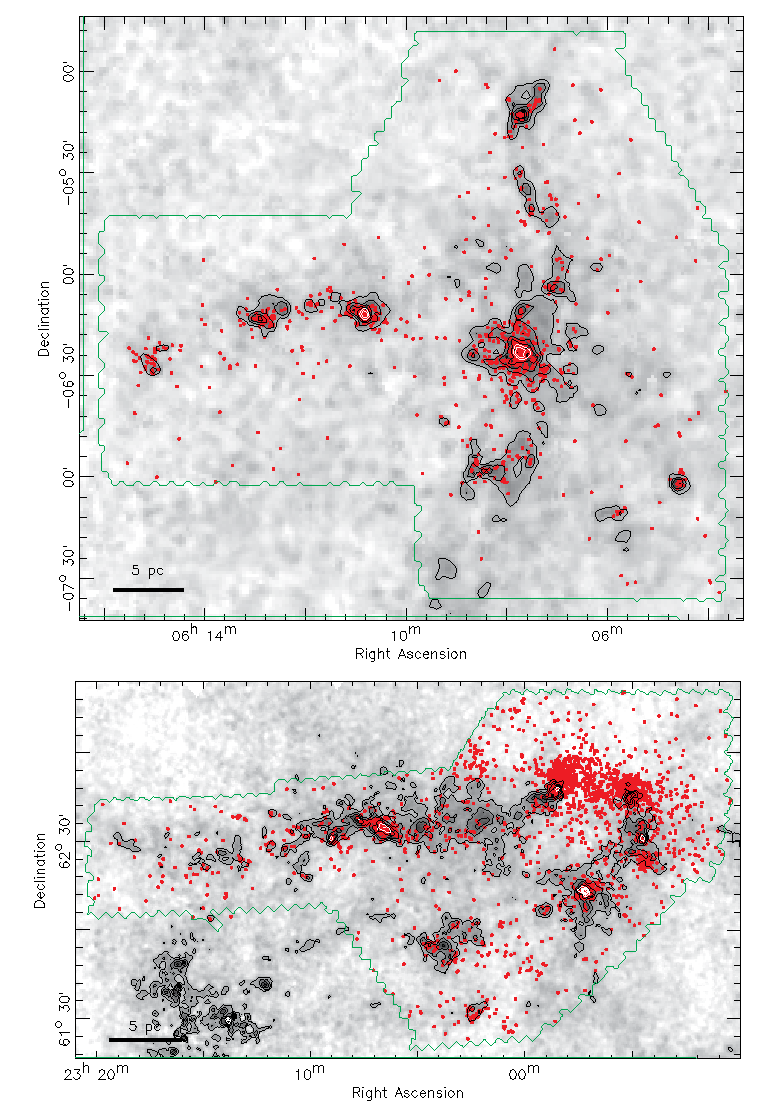
\includegraphics[width=\linewidth]{maps_gutermuth11}
\caption[Maps of gas and young stars in two clouds]{
\label{fig:maps_gutermuth11}
Maps showing the distribution of gas (grayscale) and young stellar objects (YSOs, red points) in the MonR2 (top) and CepOB3 (bottom) clouds \citep{gutermuth11a}. The grayscale gas maps are measured from dust extinction, which is plotted using a linear stretch from extinction $A_V = -1$ to 10 mag; contours start at $A_V=3$ mag, and are at 2 mag intervals.
}
\end{figure}

Such an inhomogeneous structure calls for a statistical description, and a number of statistical techniques have been used to describe gas and star arrangements. For gas we have already encountered some of these, in the form of power spectra. Power spectra can be computed for velocity structure, but they can also be computed for density structure. They can be computed for both 2D projected images of density as well as true 3D data.

Stars, on the other hand, are point objects, and so one cannot compute a power spectrum for them as one would for a continuous field like the density. However, one can compute a closely-related quantity, the two-point correlation function. Recall that, for a continuous vector field (say the velocity), we defined the autocorrelation function as
\begin{equation}
A_{\vecv}(\vecr) = \frac{1}{V} \int \vecv(\vecx) \cdot \vecv(\vecx + \vecr)\, d\vecx.
\end{equation}
For a scalar field, say density $\rho$, we can just replace the dot product with a simple multiplication. It is also common to slightly modify the definition by subtracting off the mean density so that we get a quantity that depends only on the shape of the density distribution, not its mean value. This quantity is
\begin{equation}
\label{eq:autocorr}
\xi(\vecr) = \frac{1}{V} \int [\rho(\vecx)-\overline{\rho}] [\rho(\vecx + \vecr)-\overline{\rho}]\, d\vecx,
\end{equation}
where $\overline{\rho} = (1/V) \int \rho(\vecx)\, d\vecx$. If the function is isotropic, then the autocorrelation function depends only on $r=|\vecr|$.

This is still defined for a continuous field, but we can extend the definition to the positions of a collection of point particles by imagining that the point particles represent samples drawn from an underlying probability density function. That is, we imagine that there is a continuous probability $(dP(\vecr)/dV)\, dV$ of finding a star in a volume of size $dV$ centered at some position $\vecr$, and that the actual stars present represent a random draw from this distribution.

In this case one can show that the autocorrelation function can be defined by the following procedure. Imagine drawing stellar positions from the PDF until the mean number density is $n$, and then imagine choosing a random star from this sample. Now consider a volume $dV$ that is displaced by a distance $\vecr$ from the chosen star. If $dP(\vecr)/dV$ were uniform, i.e., if there were no correlation, then the probability of finding another star at that point would simply be $n\, dV$. The two-point correlation function is then the \textit{excess} probability of finding a star over and above this value. That is, if the actual probability of finding a star is $dP_2(\vecr)/dV$, we define the two-point correlation function by
\begin{equation}
\frac{dP_2}{dV}(\vecr) = n \left[1 + \xi(\vecr)\right].
\end{equation}
Defined this way, the quantity $\xi(\vecr)$ is known as the two-point correlation function. It is possible to show that, with this definition, $\xi(\vecr)$ is equivalent to that given by equation (\ref{eq:autocorr}) applied to the underlying probability density function. As above, if the distribution is isotropic, then $\xi$ depends only on $r$, not $\vecr$. Also note that this is a 3D distribution, but if one only has 2D data on positions (the usual situation in practice), one can also define a 2D version of this where the volume is simply interpreted as representing annuli on the sky rather than shells in 3D space.

How does one go about estimating $\xi(r)$ in practice? There are a few ways. The most sophisticated is to take the measured positions and randomize them to create a random catalog, measure the numbers of object pairs in bins of separation, and use the difference between the random and true catalogs as an estimate of $\xi(r)$. This is the normal procedure in the galaxy community where surveys have well-defined areas and selection functions. In the star formation community, things are a bit more primitive, and the usual procedure is just to count the mean surface density of neighbors as a function of distance around a star, that is, to estimate that
\begin{equation}
\Sigma(r) = n \left[1 + \xi(r)\right]
\end{equation}
where $r$ is taken to be the projected separation. This is quite rough, and is vulnerable to considerable biases arising from things like edge effects (formally the correlation function is only defined over an infinite volume, but in reality of course surveys are finite in size), but it is what the star formation community generally uses.

With that formal throat-clearing out of the way, we are now in a position to look at actual data, and, since we have these clean definitions, we can talk about gas and stars on essentially equal footing. So what do autocorrelation functions of gas and star look like? Figure \ref{fig:correlation_stargas} shows some example measurements.

\begin{figure}
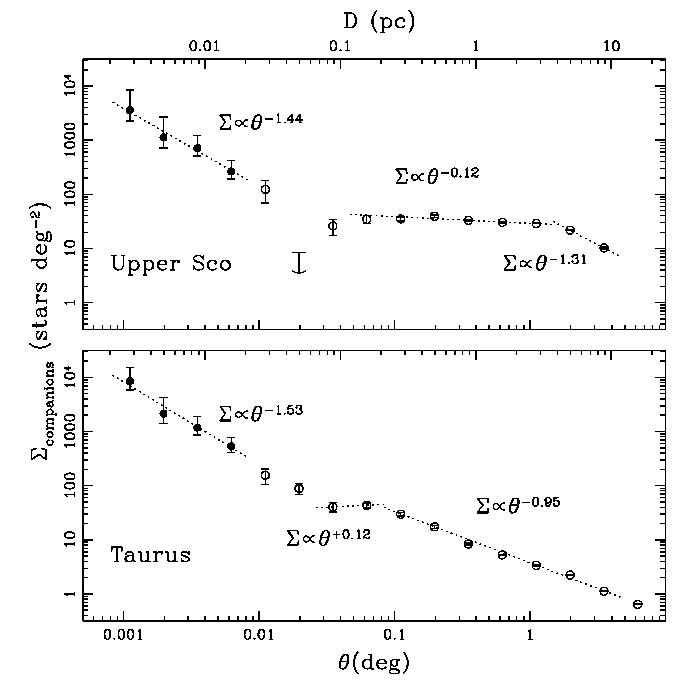
\includegraphics[height=5.2cm]{starcorrelation_kraus08}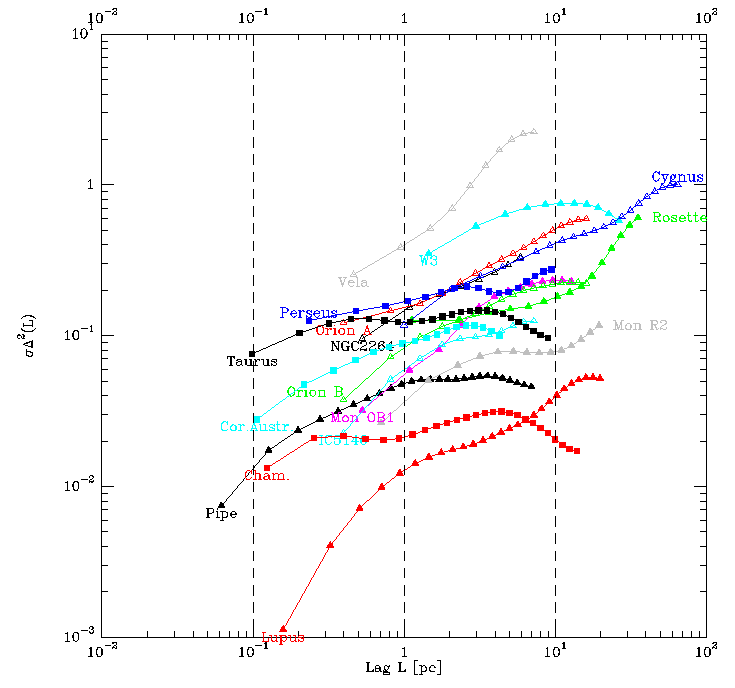
\includegraphics[height=5cm]{gascorrelation_schneider11}
\caption[Correlation functions for gas and stars]{
\label{fig:correlation_stargas}
Measurements of the stellar and gas correlations in nearby star-forming regions. The two figures on the left show the surface density of neighbors around each star $\Sigma(r)$ in Upper Sco and Taurus \citep{kraus08a}. The right panel shows measurements, for a large number of nearby molecular clouds, of a statistic called the $\Delta$ variance, $\sigma \Delta^2$, which is related to the correlation function \citep{schneider11a}.
}
\end{figure}

In the stellar distributions, we can identify a few features. At small separations, we see one powerlaw distribution. This is naturally identified as representing wide binaries. This falls off fairly steeply, until it breaks to a shallower falloff at larger separations, which can be interpreted as describing the distribution of stars within the cluster. This is also a powerlaw, covering several orders of magnitude in separation. That fact that the distribution is well fit by a powerlaw indicates that the stars follow a self-similar, scale-free structure. One can interpret such a structure as a fractal, and the index of the powerlaw is related to the dimensionality of the fractal; typical values for the dimensionality are $\sim 1$, consistent with a highly filamentary structure.

\begin{marginfigure}
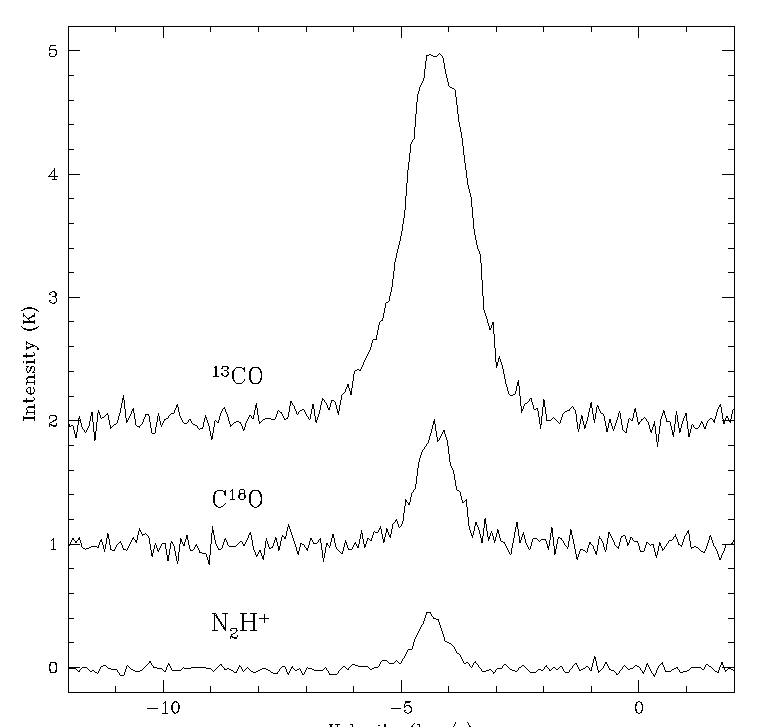
\includegraphics[width=\linewidth]{denvel_walsh04}
\caption[Velocity distributions in varying molecular lines]{
\label{fig:denvel_walsh04}
Velocity distributions measured toward a nearby protostellar core using three different molecular line tracers, as indicated. The transitions $^{13}$CO, C$^{18}$O, and N$_2$H$^+$ should be roughly ordered from lowest to highest in terms of the density of gas that produces them. From \citet{walsh04a}.
}
\end{marginfigure}

For the gas, one tends to obtain a similar powerlaw structure over a broad range of scales, with possible breaks at the high and low end. Thus the basic conclusion is that the stars and gas are in highly structured, fractal-like distributions. At young ages, the gas and stellar distributions are highly correlated with one another, which is not surprising. For older stellar populations, the correlation begins to break down.

\begin{marginfigure}
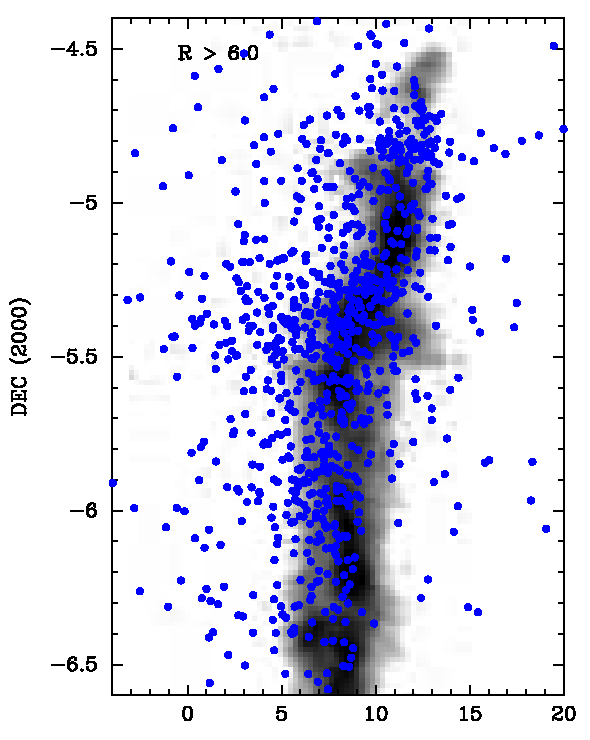
\includegraphics[width=\linewidth]{gasstar_tobin09}
\caption[Spatial and velocity distributions of gas and stars]{
\label{fig:gasstar_tobin09}
Measured distributions of $^{13}$CO (grayscale) and young stellar objects (blue points) in velocity ($x$ axis) and position on the sky in one dimension ($y$ axis) for the Orion Nebula Cluster. From \citet{tobin09a}.
}
\end{marginfigure}

In addition to the spatial distribution of stars and gas, one can also ask about their kinematics. Stellar kinematics can be determined by spectroscopy, and gas kinematics by molecular line observations. Depending on the choice of line, one learns about the kinematics of either lower or higher density regions of gas. These studies show that both the dense gas and the stars have much lower velocity dispersions than the less dense gas (Figures \ref{fig:denvel_walsh04} and \ref{fig:gasstar_tobin09}), but that the mean velocities are quite well correlated. The lower velocity dispersion will prove important below.

\subsection{Time Evolution of the Stellar Distribution}

As discussed in Chapter \ref{ch:gmcs}, stars stay associated with the gas from which they form for only a relatively short period. One can see this transition directly by comparing older and younger stellar populations. The younger the stellar population, the better the star-gas correlation. By stellar ages of $\sim 5-10$ Myr, there is usually no associated gas at all. However, it is still interesting to investigate how the stars evolve, because this contains important clues about how the formed.

The typical star-forming environment is vastly denser than the mean of the ISM, and as a result the stars that form are also vastly denser, in terms of either mass or number of stars per unit volume, than the mean density of gas in the ISM or stars near the Galactic midplane. More than 90\% of star formation observed within 2 kpc of the Sun takes place in regions where the stellar mass density exceeds $1$ $M_\odot$ pc$^{-3}$, corresponding to a number density $n > 30$ cm$^{-3}$ \citet{lada03a}. In comparison, the stellar mass density in the Solar neighborhood is $\sim 0.01$ $M_\odot$ pc$^{-3}$ \citep{holmberg00a}), and the mean density of gas in the ISM is $\sim 1$ cm$^{-3} \approx 0.03$ $M_\odot$ pc$^{-3}$.

However, these high densities do not last. If one examines stars at an age of $\sim 100$ Myr, the ratio is flipped -- only $\sim 10\%$ are in star clusters with a density identifiably higher than that of the stellar field, while $\sim 90\%$ have dispersed and can no longer be identified as members of discrete clusters (Figure \ref{fig:clusterage_fall12}). (They can, however, still be grouped by their kinematics, which take much longer to be randomized than their positions. Collections of stars that are now at low density and no longer show up as clusters based on their positions, but that remain very close together in velocity space, are called moving groups.)

\begin{marginfigure}
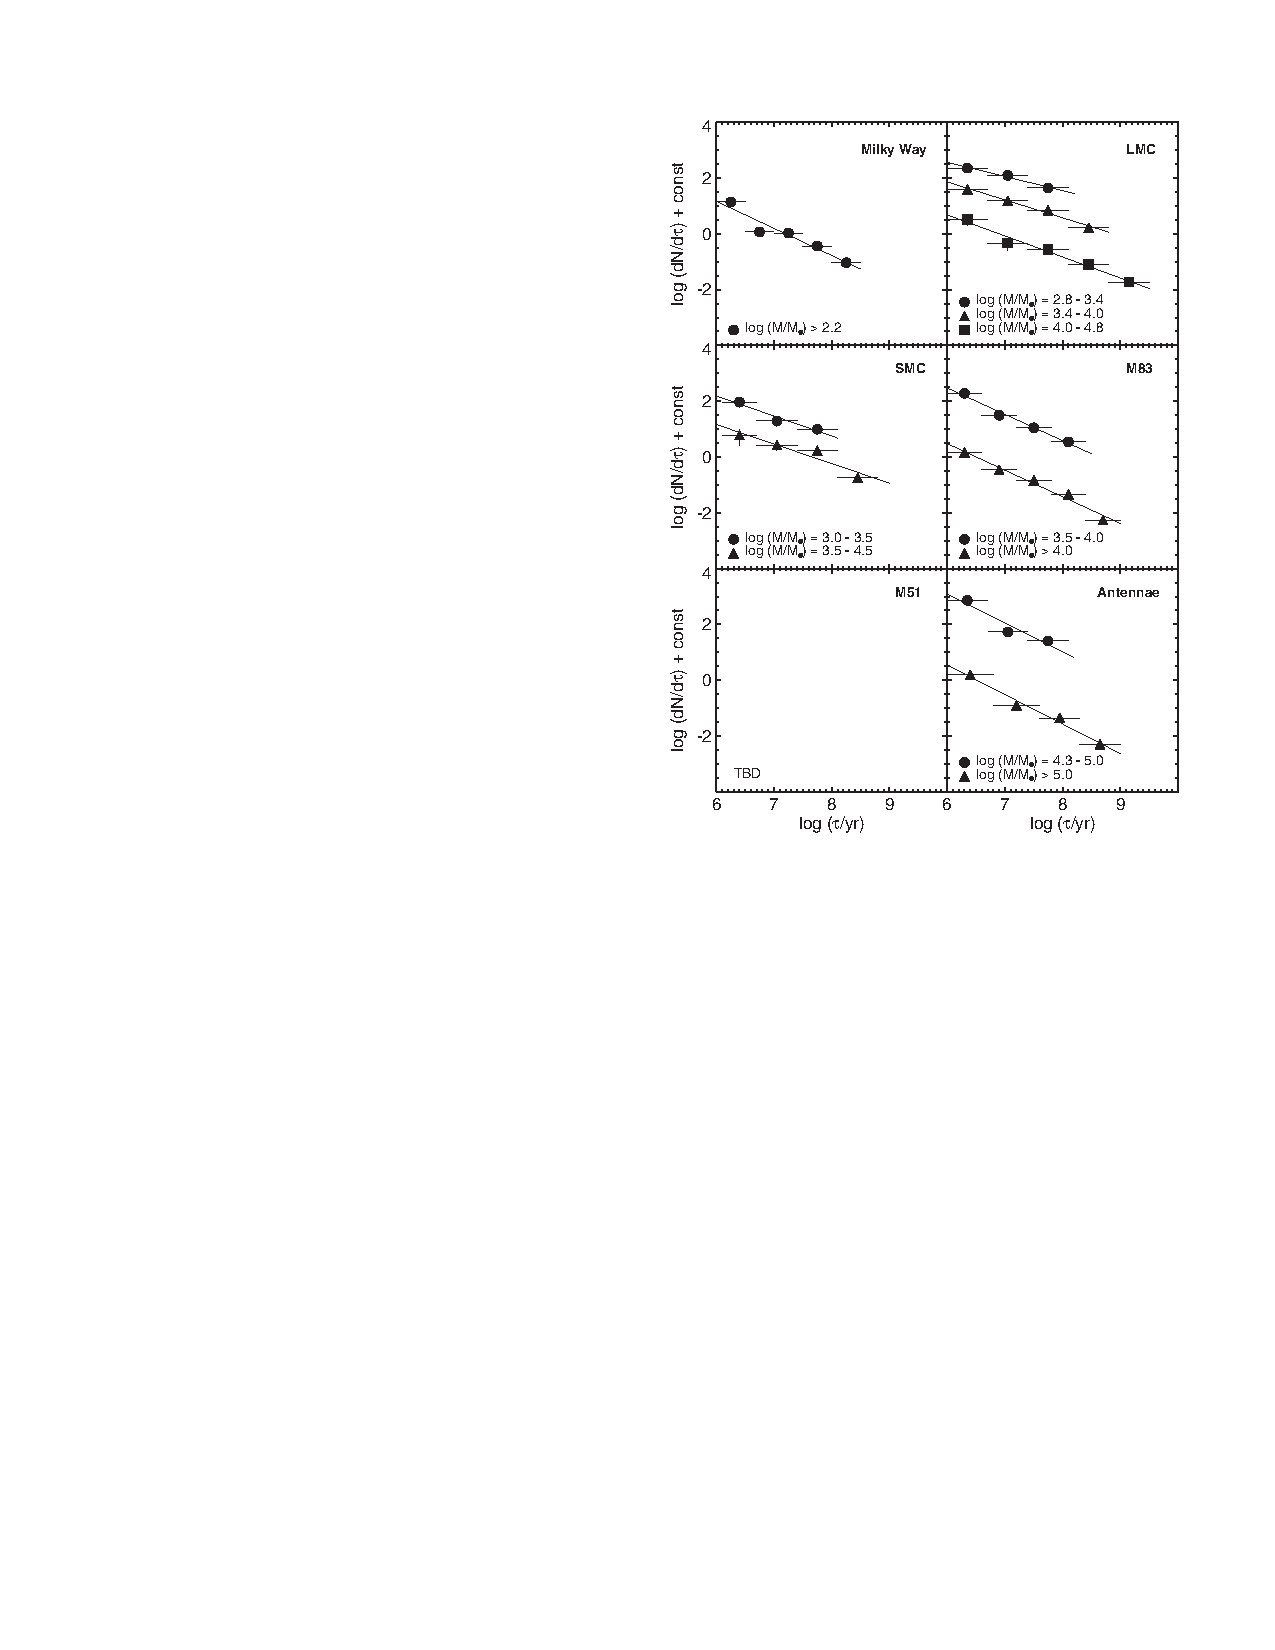
\includegraphics[width=\linewidth]{clusterage_fall12}
\caption[Star cluster age distributions]{
\label{fig:clusterage_fall12}
Measured distributions of star cluster ages in several galaxies \citep{fall12a}. Clusters have been binned in mass, and different symbols show different mass bins, as indicated.
}
\end{marginfigure}

The exact functional form of this decline in number of star clusters, and whether the fraction that remain in clusters after some period of time varies with the large-scale properties of the galaxy, are both uncertain. The answers seems to depend at least in part on how one chooses to define "cluster" at very young ages when the stars are still in a fractal, non-relaxed distribution. Nonetheless, the fact that the stars disperse tells us something very important, which is that they must have formed via a mechanism that leaves the resulting stellar system gravitationally unbound. Only in very rare cases does a bound stellar system remain after the gas is removed. This is an important constraint for theories of star formation.

\begin{marginfigure}
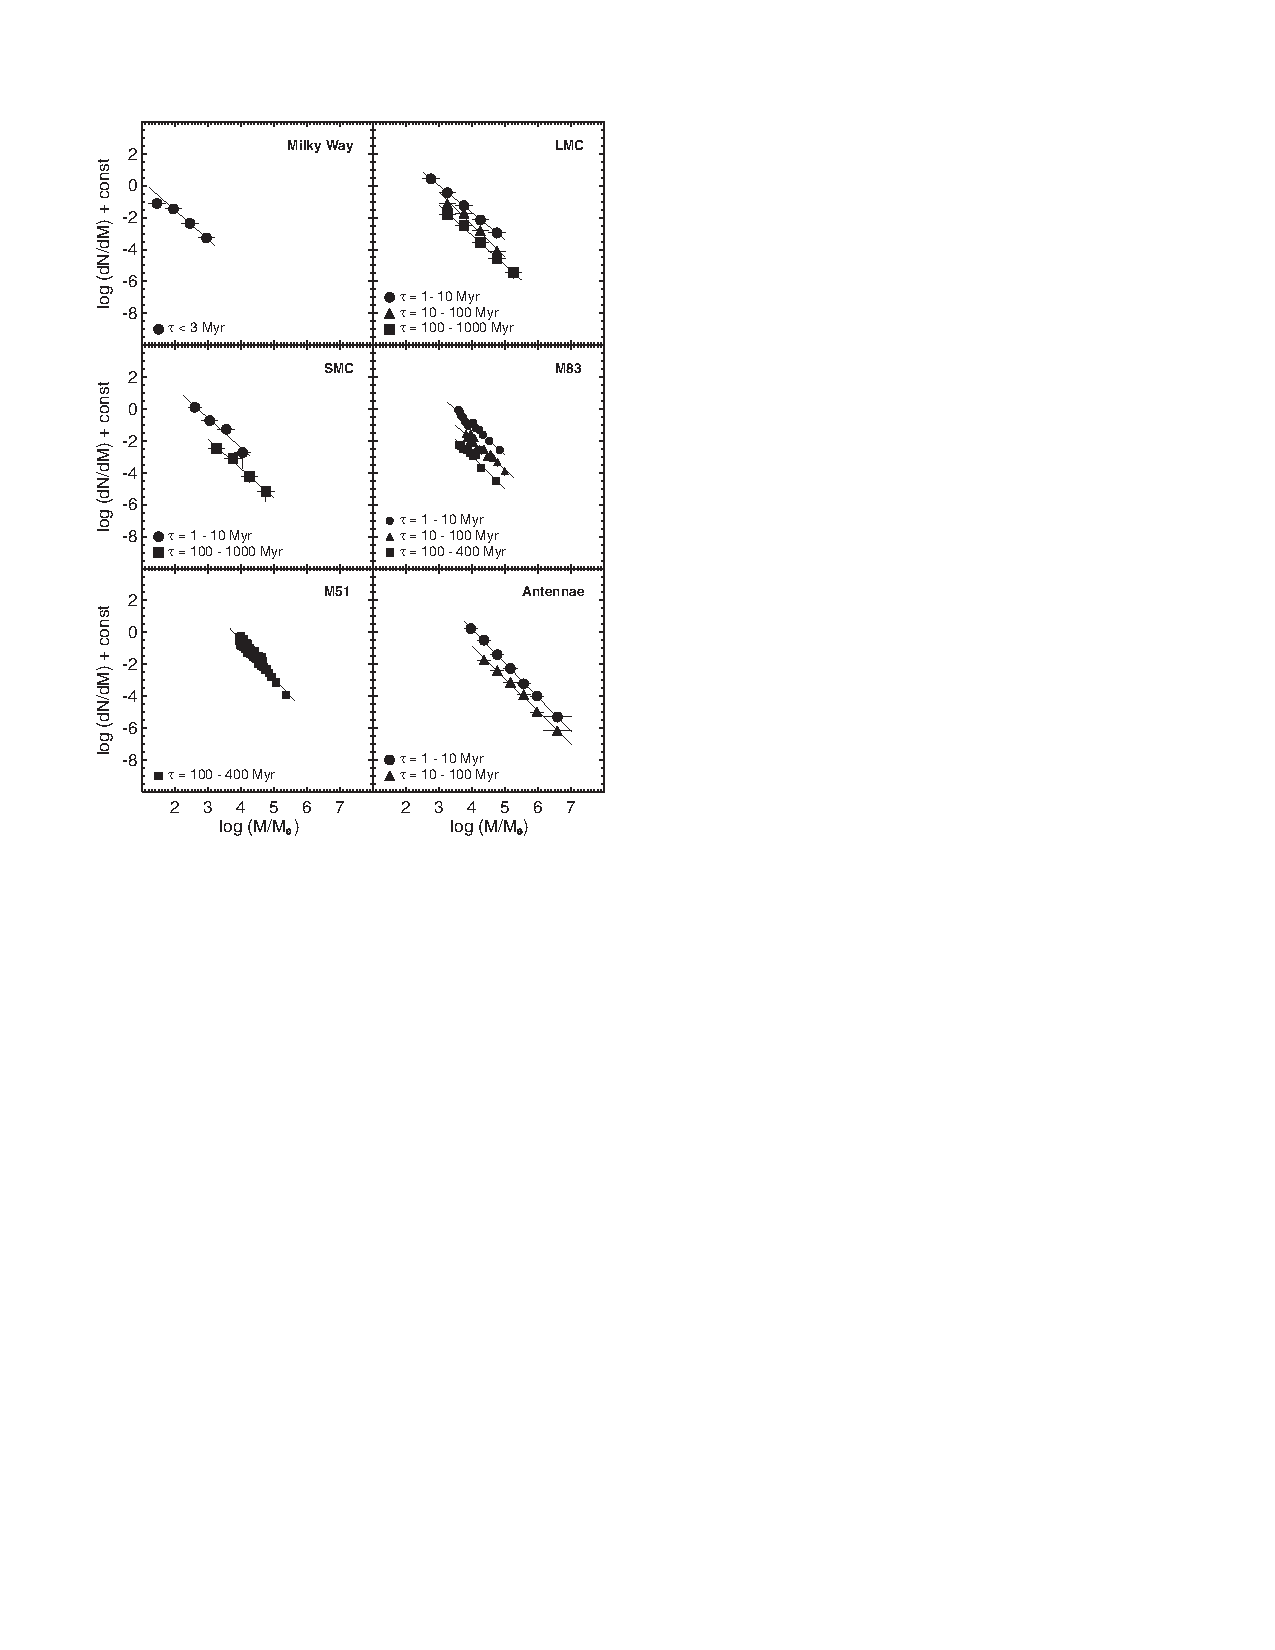
\includegraphics[width=\linewidth]{clustermass_fall12}
\caption[Star cluster mass distributions]{
\label{fig:clustermass_fall12}
Measured distributions of star cluster mass in several galaxies \citep{fall12a}. Clusters have been binned in age, and different symbols show different age bins, as indicated.
}
\end{marginfigure}

A second important observational constraint is that the star clusters that do remain always show mass distribution that is close to a powerlaw of the form $dN/dM \propto M^{-2}$ (Figure \ref{fig:clustermass_fall12}), meaning equal mass per logarithmic bin in cluster mass. This mass function is recovered in essentially all galaxies that have been examined, and does not appear to vary with large-scale galaxy properties. The origin of this distribution is also currently debated.


\section{Theory of Stellar Clustering}

Having discussed the observational situation, we now turn to theoretical models for the origin of stellar clustering. The models here are somewhat less developed than for either the star formation rate or the IMF, but the problem is no less important and interesting.

\subsection{Origin of the Gas and Stellar Distributions}

The origin of the spatial and kinematic distributions of gas and stars, and the correlation between them, ultimately seems to lie in very general behaviors of cold gas. The characteristic timescale for gravitational collapse is the free-fall time, which varies with density as $t_{\rm ff} \propto \rho^{-1/2}$. As a result, the densest regions tend to run away and form stars first, leading a a highly structured distribution in which stars are concentrated in the densest regions of gas. Quantitatively, simulations of turbulent flows are able to reproduce the powerlaw-like two point correlation functions that are observed \citep{hansen12a}.

\begin{marginfigure}
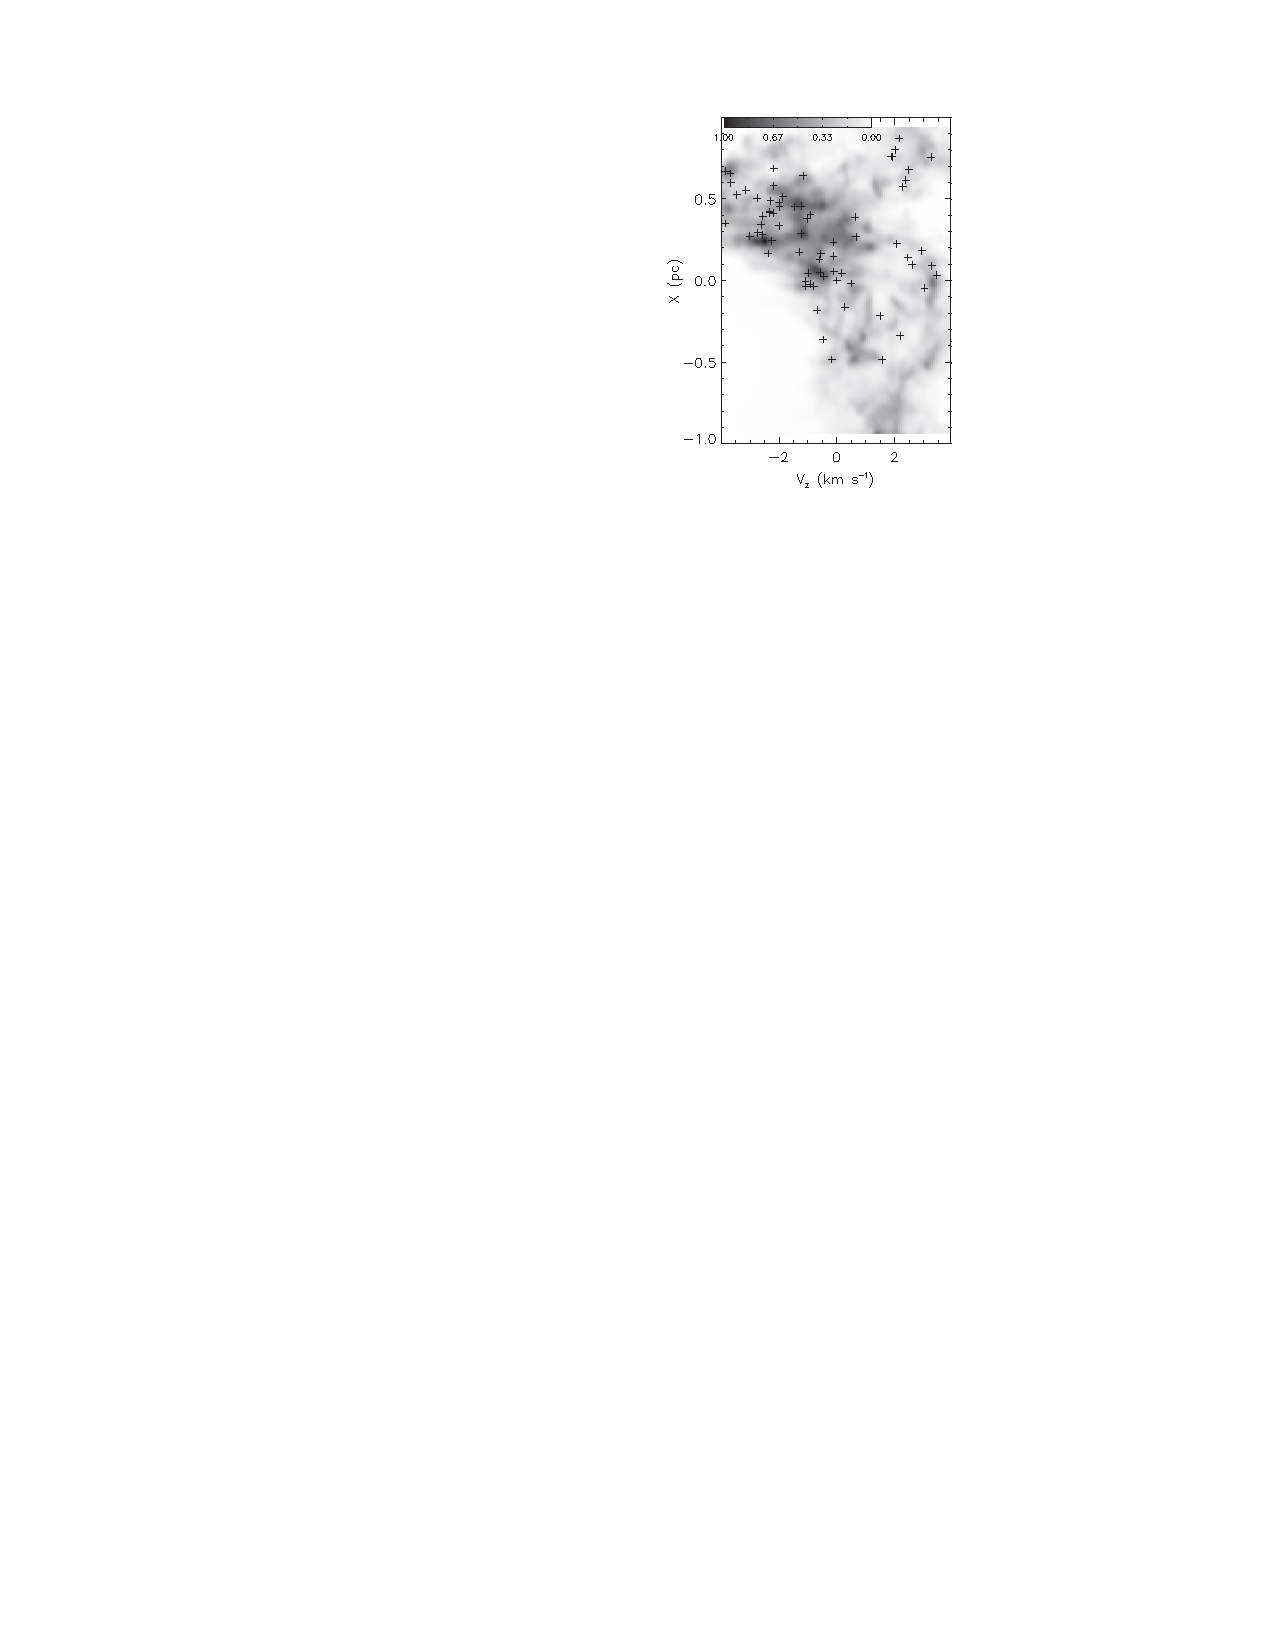
\includegraphics[width=\linewidth]{gasstar_offner09}
\caption[Spatial and velocity distributions of gas and stars in a simulation]{
\label{fig:gasstar_offner09}
Distributions of $^{13}$CO (grayscale) and young stellar objects (black crosses) in velocity ($x$ axis) and position on the sky in one dimension ($y$ axis) in a simulation of the Orion Nebula Cluster \citep{offner09b}.
}
\end{marginfigure}

The kinematics also arise from the properties of cold, turbulent gas. One general feature of such flows is a density-velocity anti-correlation. The densest regions of gas are produced by strong converging shocks, and immediately after the passage of such a shock the velocity is small because of the cancellation of opposing fluid velocities. The stars form from these dense, shocked regions, and so they inherit the low velocities of the dense gas out of which they form -- in some sense the stars are simply the tip of the density distribution. Again, simulations can qualitatively and quantitatively reproduce the observed kinematics. Figure \ref{fig:gasstar_offner09} shows an example.

\subsection{Gas Removal and the Transition to Gas-Free Evolution}

It seems that the spatial and kinematic arrangements of young stars are understood reasonably well. This is mainly because the physics that is responsible for them -- gravity plus hydrodynamics -- is well understood and easy to simulate.  Where we start to run into trouble is when we try to follow the transition from gas-dominated to gas-free evolution, where stellar feedback almost certainly plays a role.

First of all, as a baseline, let us consider what happens if we do not include any feedback. We have already seen that this creates dimensionless star formation rates $\epsilon_{\rm ff}$ that are $\sim 2$ orders of magnitude too high. However, omitting feedback also leads to problems when it comes to stellar clustering, because if one omits feedback, then most of the available gas is transformed into stars. The result is that, if the gas cloud from which the stars formed was bound to begin with, the resulting stellar system is also bound, and thus all star formation occurs in bound clusters.

In fact, the situation is even worse than that: even if one starts with an \textit{unbound} gas cloud, then if star formation feedback does not prevent consumption of most of the gas, the result is still that most of the stars are members of bound clusters. This happens because most of the kinetic energy is on large scales, so that, even if the entire cloud is unbound, there are plenty of sub-regions within it that become bound as the turbulence dissipates \citep{clark04a}. The result is that unbound clouds wind up fragmenting into a few clusters that are unbound from one another, but that are at internally bound. Thus explaining the observed fact that most stars are not members of bound clusters requires some mechanism to truncate star formation well before the majority of the mass is transformed to stars. 

\paragraph{Rapid Versus Adiabatic Mass Loss}

To see what fraction of the gas mass must be lost to render the system unbound, we can begin with a simple argument. Let us consider a system of gas and stars with total mass $M$ in virial equilibrium, and with negligible support from magnetic fields. In this case, we have
\begin{equation}
2\mathcal{T} + \mathcal{W} = 0,
\end{equation}
where $\mathcal{T}$ is the total thermal plus kinetic energy, and $\mathcal{W}$ is the gravitational potential energy. Now let us consider what happens if we remove mass from the system, reducing the mass from $M$ to $\epsilon M$. We can envision that this is because a fraction $\epsilon$ of the starting gas mass has been turned into stars, while the remaining fraction $1-\epsilon$ is in the form of gas that is removed by some form of stellar feedback.

First suppose the removal is very rapid, on a timescale much shorter than the crossing time or free-fall time. In this case there will be no time for the system to adjust, and all the particles that remain will keep the same velocity and temperature. Thus the new kinetic energy is
\begin{equation}
\mathcal{T}' = \epsilon \mathcal{T}.
\end{equation}
Similarly, the positions of all particles that remain will be unchanged, so if the mass removal is uniform (i.e., we remove mass by randomly removing a certain fraction of the particles, without regard for their location) then the new potential energy will be
\begin{equation}
\mathcal{W}' = \epsilon^2 \mathcal{W}.
\end{equation}
The total energy of the system after mass removal is
\begin{equation}
E' = \mathcal{T}' + \mathcal{W'} = \epsilon \mathcal{T} + \epsilon^2 \mathcal{W} = \epsilon(1-2\epsilon) \mathcal{T} = \epsilon\left(\epsilon-\frac{1}{2}\right) \mathcal{W}
\end{equation}
Since $\mathcal{T} > 0$ and $\mathcal{W} < 0$, it immediately follows that the total energy of the system after mass removal is negative if and only if $\epsilon > 1/2$. Thus the system remains bound only if we remove less than $1/2$ the mass, and becomes unbound if we remove more than $1/2$ the mass. 

If the system remains bound, it will eventually re-virialize at a new, larger radius. We can solve for this radius from the equations we have already written down. The total energy of a system in virial equilibrium is
\begin{equation}
E = \frac{\mathcal{W}}{2} = -a\frac{GM^2}{2R},
\end{equation}
so if the system re-virializes the new radius $R'$ must obey
\begin{equation}
E' = -a\frac{G(\epsilon M)^2}{2R'}.
\end{equation}
However, we also know that
\begin{equation}
E' = \epsilon\left(\epsilon-\frac{1}{2}\right) \mathcal{W} = -\epsilon\left(\epsilon-\frac{1}{2}\right)a\frac{GM^2}{R},
\end{equation}
and combining these two statements we find that the new radius is
\begin{equation}
R' = \frac{\epsilon}{2\epsilon-1} R.
\end{equation}

Now consider the opposite limit, where mass is removed very slowly compared to the crossing time. To see what happens in this case, it is helpful to imagine the mass loss as occurring in very small increments, and after each increment of mass loss waiting for the system to re-establish virial equilibrium before removing any more mass. Such mass loss if referred to as adiabatic. If we change the mass by an amount $dM$ (with the sign convention that $dM < 0$ indicates mass loss), we can find the change in radius $dR$ by Taylor expanding the equation we just derived for the new radius, recalling that $\epsilon = 1 + dM/M$:
\begin{equation}
R' = \frac{\epsilon}{2\epsilon-1} R = \frac{1 + dM/M}{1 + 2 dM/M} R = \left[1 - \frac{dM}{M} + O\left(\frac{dM^2}{M^2}\right)\right] R
\end{equation}
Thus
\begin{equation}
\frac{dR}{R} = \frac{R' - R}{R} = -\frac{dM}{M},
\end{equation}
and if we integrate both sides then we obtain
\begin{equation}
\ln R = -\ln M + \mbox{const} \qquad\Longrightarrow\qquad R' \propto \frac{1}{M}.
\end{equation}
Thus if we reduce the mass from $M$ to $\epsilon M$ but do it adiabatically, the radius changes from $R$ to $R/\epsilon$. The system remains bound at all times, and just expands smoothly.

These simple arguments would suggest that mass loss should produce a bound cluster if the star formation efficiency is $>1/2$ and or the mass removal is slow, and an unbound set of stars if the efficiency is $<1/2$ and the mass removal is fast. In reality, life is more complicated than these simple arguments suggest, for a few reasons.

First, even if gas removal is rapid, some stars will still become unbound even if $\epsilon > 1/2$, and some will still remain bound even if $\epsilon < 1/2$. This is because the energy is not perfectly shared among the stars. Instead, at any given instant, some stars are moving faster than their average speed, and some are moving slower. Those that are moving rapidly at the instant when mass is removed will simply sail on out of the much-reduced potential well without sharing their energy, and thus can be lost even if $\epsilon > 1/2$. Conversely, the slowest-moving stars will not escape even if there is a very large reduction in the potential well, because they will not have time to acquire energy from the faster stars that escape. Thus for rapid mass loss, there is not a sharp boundary at $\epsilon = 1/2$. Instead, there is more of a smooth transition from no stars becoming unbound at $\epsilon \sim 1$ to no stars remaining at $\epsilon \sim 0$.

Second, we have done our calculations in a vacuum, but in reality star clusters exist inside a galactic potential, and this creates a tidal gravitational field. If a star wanders too far from the cluster, the tidal field of the galaxy will pull it off. Thus our conclusion that, in the adiabatic case, the cluster always remains bound and simply expands, must fail once the expansion proceeds too far. The outermost parts of the cluster will start to be stripped if they expand too far, and if the expansion proceeds so far that the mean density of the cluster becomes too low, it will be pulled apart entirely.

Third, the calculation we have just gone through assumes that the system starts in virial equilibrium, with the stars moving at the speed expected for virial balance. However, as we discussed before, this is not a good assumption: the stars have a much lower velocity dispersion than the gas when the cluster is young, and thus are much harder to unbind than the above argument suggests. If star formation continues for more than a single crossing time, this should become less and less of a problem as time passes and the stars are able to relax and dynamically heat up in the potential well of the gas. However, if star formation is ended very rapidly, in a crossing time, then the efficiency will have to be even lower than the value we have just estimated to be able to unbind the stars, since they are starting from much lower kinetic energies than they would have in virial balance.

\paragraph{The Cluster Formation Efficiency}

Given the theoretical modeling we have just performed, what can we say about what fraction of star formation will result in bound stellar clusters that will survive the initial gas expulsion? To address this question, we must be able to calculate the star formation efficiency, which is of course a very difficult problem, quite analogous to the problem of understanding what limits the rate of star formation overall. The answer almost certainly involves some sort of stellar feedback, so we can study a simple model for how that might work, drawn from \citet{fall10a}.

Let us consider a spherical gas cloud of initial mass $M$ and radius $R$, which begins forming stars. Star formation ends when the stars are able to inject momentum into the remaining gas at a rate high enough to raise that gas to a speed of order the escape speed in a time comparable to the crossing time. The requisite speed is
\begin{equation}
v_e \sim \sqrt{\frac{G M}{R}}.
\end{equation}
If the stellar mass at any given time is $\epsilon M$, then the momentum injection rate is
\begin{equation}
\dot{p} = \left\langle\frac{\dot{p}}{M_*}\right\rangle \epsilon M,
\end{equation}
where the quantity in angle brackets is momentum per unit time per unit stellar mass provided by a zero age population of stars. Thus our condition is that star formation ceases when
\begin{equation}
M v_e \sim \dot{p} t_{\rm cr} \sim \left\langle\frac{\dot{p}}{M_*}\right\rangle \epsilon M \frac{R}{v_e},
\end{equation}
where, since we are dropping factors of order unity, we have simply taken $t_{\rm cr} \sim R/v_e$.

Re-arranging, we conclude that star formation should cease and gas should be expelled when
\begin{equation}
\epsilon \sim \left\langle\frac{\dot{p}}{M_*}\right\rangle^{-1} \frac{v_e^2}{R} \sim \left\langle\frac{\dot{p}}{M_*}\right\rangle^{-1} G\Sigma,
\end{equation}
where $\Sigma \sim M/R^2$ is the surface density of the cloud.

Thus we expect to achieve a star formation efficiency of $\epsilon \sim 0.5$ when
\begin{equation}
\left\langle\frac{\dot{p}}{M_*}\right\rangle\sim G \Sigma.
\end{equation}
Just to give a sense of what this implies, we showed in \autoref{ch:feedback} that $\left\langle\dot{p}/M_*\right\rangle$ for stellar radiation is 23 km s$^{-1}$ Myr$^{-1}$, and plugging this in we obtain $\Sigma \sim 1$ g cm$^{-2}$. Thus regions with surface densities of $\sim 1$ g cm$^{-2}$ should be able to form bound clusters, while those with lower surface densities should not. This might plausibly explain why most regions do not form bound clusters.

However, this is an extremely crude calculation, and it assumes that one can define a well-defined "cloud" with a well-defined surface density. Real clouds, of course, have complex fractal structures. The suggested literature reading for this chapter, \citet{kruijssen12a}, is an attempt to develop a theory somewhat like this for a more realistic model of the structure of a cloud.

\paragraph{The Cluster Mass Function}

As a final topic for this chapter, what are the implications of this sort of analysis for the cluster mass function? Again, we will proceed with a spherical cow style of analysis. Consider a collection of star-forming gas clouds with an observed mass spectrum $dN_{\rm obs}/dM_g$. Each such cloud lives for a time $t_\ell(M_g)$ before forming its stars and dispersing, so the cluster formation rate is
\begin{equation}
\frac{dN_{\rm form}}{dM_g} \propto \frac{1}{t_{\ell}(M_g)} \frac{dN_{\rm obs}}{dM_g}.
\end{equation}

Now let $\epsilon$ be the final star formation efficiency for a cloud of mass $M_g$, and let $f_{\rm cl}(\epsilon)$ be the fraction of the stars that remain bound following gas removal. Thus the final mass of the star cluster formed will be
\begin{equation}
M_c = f_{\rm cl} \epsilon M_g.
\end{equation}
From this we can calculate the formation rate for star clusters of mass $M_c$:
\begin{eqnarray}
\frac{dN_{\rm form}}{dM_c} & = & \left(\frac{dM_c}{dM_g}\right)^{-1} \frac{dN_{\rm form}}{dM_g} \\
& \propto & \left[\epsilon f_{\rm cl} + \left(f_{\rm cl}+ \frac{df_{\rm cl}}{d\ln \epsilon}\right) \frac{d\epsilon}{d\ln M_g}\right]^{-1} 
\nonumber \\
& & {} \cdot
\frac{1}{t_{\ell}(M_g)} \frac{dN_{\rm obs}}{dM_g}.
\end{eqnarray}

Let us unpack this result a bit. It tells us how to translate the observed cloud mass function into a formation rate for star clusters of different masses. This relationship depends on several factors. The factor $1/t_\ell(M_g)$ simply accounts for the fact that our observed catalog of clouds oversamples the clouds that stick around the longest. The factor $\epsilon f_{\rm cl}$ just translates from gas cloud mass to cluster mass. The remaining factor, $(f_{\rm cl} + df_{\rm cl}/d\ln\epsilon)(d\epsilon/d\ln M_g)$, compensates for the way the gas cloud mass function gets compressed or expanded due to any non-linear mapping between gas cloud mass and final star cluster mass. The mapping will be non-linear if the star formation efficiency is not constant with gas cloud mass, i.e., if $d\epsilon/d\ln M_g$ is non-zero.

Since observed gas cloud mass functions are not too far from the $dN/dM \propto M^{-2}$ observed for the final star cluster mass function, this implies that the terms in square brackets cannot be extremely strong functions of $M_g$. This is interesting, because it implies that the star formation efficiency $\epsilon$ cannot be a very strong function of gas cloud mass.
